\documentclass[12pt]{article}
\usepackage{geometry} % Pour passer au format A4
\geometry{hmargin=1cm, vmargin=1cm} % 

% Page et encodage
\usepackage[T1]{fontenc} % Use 8-bit encoding that has 256 glyphs
\usepackage[english,french]{babel} % Français et anglais
\usepackage[utf8]{inputenc} 

\usepackage{lmodern}
\setlength\parindent{0pt}

% Graphiques
\usepackage{graphicx,float,grffile}

% Maths et divers
\usepackage{amsmath,amsfonts,amssymb,amsthm,verbatim}
\usepackage{multicol,enumitem,url,eurosym,gensymb}

% Sections
\usepackage{sectsty} % Allows customizing section commands
\allsectionsfont{\centering \normalfont\scshape}

% Tête et pied de page

\usepackage{fancyhdr} 
\pagestyle{fancyplain} 

\fancyhead{} % No page header
\fancyfoot{}

\renewcommand{\headrulewidth}{0pt} % Remove header underlines
\renewcommand{\footrulewidth}{0pt} % Remove footer underlines

\newcommand{\horrule}[1]{\rule{\linewidth}{#1}} % Create horizontal rule command with 1 argument of height

%----------------------------------------------------------------------------------------
%	Début du document
%----------------------------------------------------------------------------------------

\begin{document}

%----------------------------------------------------------------------------------------
% RE-DEFINITION
%----------------------------------------------------------------------------------------
% MATHS
%-----------

\newtheorem{Definition}{Définition}
\newtheorem{Theorem}{Théorème}
\newtheorem{Proposition}{Propriété}

% MATHS
%-----------
\renewcommand{\labelitemi}{$\bullet$}
\renewcommand{\labelitemii}{$\circ$}
%----------------------------------------------------------------------------------------
%	Titre
%----------------------------------------------------------------------------------------

\setlength{\columnseprule}{1pt}

\section*{IE1 - Statistiques}
\horrule{2px}

\begin{multicols}{2}

\subsection*{Restituer}

Donner une définition de la médiane. 

\horrule{1px}
\subsection*{Ex1 - Représenter}

\begin{enumerate}
\item[1.] \textsc{M. Lafond} interroge les élèves de troisième pour savoir combien de téléphones portables possèdent-ils par famille.

\begin{center}
  \begin{tabular}{|c||c|c|c|c|c|c|}
    \hline
    Nombre de portables & 0 & 1 & 2 & 3 & 4 & 5 \\
    \hline 
    Effectif & 2 & 8 & 18 & 35 & 0 & 4 \\
    \hline
  \end{tabular}
\end{center}

\textbf{Représenter} le tableau par un diagramme en bâton.

\item[2.] Voici le nombre de frères et sœurs pour chaque élève de la classe de 303 : 

$0, 1, 2, 0, 0, 2, 2, 4, 5, 2, 3, 1, 4, 7, 2, 2, 0, 1, 1, 2, 3.$

Après, avoir ranger les données dans un tableau d'effectif, \textbf{représenter} les données dans un diagramme en bâton.
\end{enumerate}

\horrule{1px}
\subsection*{Ex2 - Notes}

Yanice a obtenu les notes suivantes aux quatre premiers contrôles de SVT : 12/20, 4/20, 9/20, 11/20.

\begin{enumerate}
\item[1.] \textbf{Calculer} la moyenne de ses notes.
\item[2.] \textbf{Calculer} la note qu'il doit obtenir au $5^e$ contrôle pour que sa moyenne augmente d'un point.
\item[3.] Le annonce que le $5^e$ contrôle est coefficient 2. Yanice obtient 15/20 (\textit{Yeah !}). \textbf{Calculer} sa nouvelle sa moyenne ?
\end{enumerate}

\horrule{1px}
\subsection*{Ex3 - Planches}

Une machine sert à fabriquer des planches de 2 cm d'épaisseur. Pour savoir si la machine est bien réglé, le menuisier prélève au hasard 50 planches et mesure leurs épaisseurs.

\begin{center}
  \begin{tabular}{|c||c|c|c|c|c|c|}
    \hline
    Épaisseur (en cm)   & 1,8 & 1,9 & 2,0 & 2,1 & 2,2 & 2,3 \\
    \hline 
    Effectif & 3 & 5 & 23 & 15 & 3 & 1 \\
    \hline
  \end{tabular}
\end{center}

\begin{enumerate}
\item[1.] \textbf{Calculer} l'épaisseur moyenne des cinquante planches.
\item[2.] La machine est bien réglée si moins de $10\%$ des planches ont plus de 1mm d'écart avec l'épaisseur voulue. La machine est-elle bien réglée ? \textbf{(Raisonner)}
\end{enumerate}

\horrule{1px}
\subsection*{Ex4 - Course à pied}

Lors d'un sprint de 200m au collège, les professeurs ont obtenu ces temps : 20,15s ; 20,22s ; 20,58s, 20,09s ; 20,79s ; 20,29s ; 20,48s.

\begin{enumerate}
\item[1.] \textbf{Calculer} l'étendue de la série.
\item[2.] \textbf{Calculer} la moyenne de la série.
\item[3.] \textbf{Calculer} la médiane de la série. (Justifier)
\end{enumerate}

\horrule{1px}
\subsection*{Ex5 - Salaire}

Voici les salaires de \textsc{M. Lafond} ses six derniers mois : 2200 \euro, 2100\euro, 1800\euro, 2400\euro, 2200\euro, 1700\euro.

\begin{enumerate}
\item[1.] \textbf{Calculer} l'étendue de la série.
\item[2.] \textbf{Calculer} la moyenne de la série.
\item[3.] \textbf{Calculer} la médiane de la série. (Justifier)
\end{enumerate}

\horrule{1px}
\subsection*{Bonus - Traduire}

\begin{figure}[H]
	\centering
	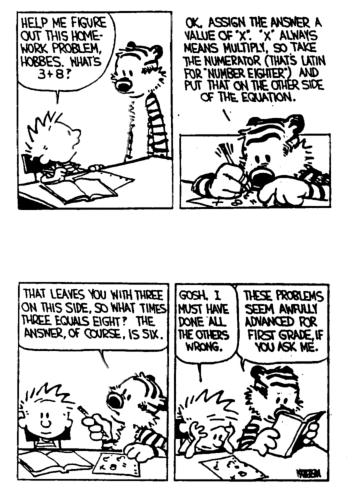
\includegraphics[width=0.7 \linewidth]{3x1-statistiques/sources/cah.jpg}
\end{figure}
\end{multicols}

\newpage

\section*{IE1 - Statistiques}
\horrule{2px}

\begin{multicols}{2}

\subsection*{Restituer}

Donner une définition de la médiane. 

\horrule{1px}
\subsection*{Ex1 - Représenter}

\begin{enumerate}
\item[1.] \textsc{M. Lafond} interroge les élèves de troisième pour savoir combien de téléphones portables possèdent-ils par famille.

\begin{center}
  \begin{tabular}{|c||c|c|c|c|c|c|}
    \hline
    Nombre de portables & 0 & 1 & 2 & 3 & 4 & 5 \\
    \hline 
    Effectif & 2 & 8 & 38 & 25 & 0 & 3 \\
    \hline
  \end{tabular}
\end{center}

\textbf{Représenter} le tableau par un diagramme en bâton.

\item[2.] Voici le nombre de frères et sœurs pour chaque élève de la classe de 303 : 

$0, 1, 2, 0, 0, 2, 2, 4, 5, 3, 4, 2, 5, 7, 1, 1, 0, 1, 1, 2, 3.$

Après, avoir ranger les données dans un tableau d'effectif, \textbf{représenter} les données dans un diagramme en bâton.
\end{enumerate}

\horrule{1px}
\subsection*{Ex2 - Notes}

Yanis a obtenu les notes suivantes aux quatre premiers contrôles de SVT : 13/20, 3/20, 8/20, 12/20.

\begin{enumerate}
\item[1.] \textbf{Calculer} la moyenne de ses notes.
\item[2.] \textbf{Calculer} la note qu'il doit obtenir au $5^e$ contrôle pour que sa moyenne augmente d'un point.
\item[3.] Le annonce que le $5^e$ contrôle est coefficient 2. Yanice obtient 16/20 (\textit{Yeah !}). \textbf{Calculer} sa nouvelle sa moyenne ?
\end{enumerate}

\horrule{1px}
\subsection*{Ex3 - Planches}

Une machine sert à fabriquer des planches de 2 cm d'épaisseur. Pour savoir si la machine est bien réglé, le menuisier prélève au hasard 50 planches et mesure leurs épaisseurs.

\begin{center}
  \begin{tabular}{|c||c|c|c|c|c|c|}
    \hline
    Épaisseur (en cm)   & 1,8 & 1,9 & 2,0 & 2,1 & 2,2 & 2,3 \\
    \hline 
    Effectif & 3 & 5 & 15 & 23 & 3 & 2 \\
    \hline
  \end{tabular}
\end{center}

\begin{enumerate}
\item[1.] \textbf{Calculer} l'épaisseur moyenne des cinquante planches.
\item[2.] La machine est bien réglée si moins de $10\%$ des planches ont plus de 1mm d'écart avec l'épaisseur voulue. La machine est-elle bien réglée ? \textbf{(Raisonner)}
\end{enumerate}

\horrule{1px}
\subsection*{Ex4 - Course à pied}

Lors d'un sprint de 200m au collège, les professeurs ont obtenu ces temps : 20,15s ; 20,24s ; 20,56s, 20,07s ; 20,77s ; 20,27s ; 20,46s.

\begin{enumerate}
\item[1.] \textbf{Calculer} l'étendue de la série.
\item[2.] \textbf{Calculer} la moyenne de la série.
\item[3.] \textbf{Calculer} la médiane de la série. (Justifier)
\end{enumerate}

\horrule{1px}
\subsection*{Ex5 - Salaire}

Voici les salaires de \textsc{M. Lafond} ses six derniers mois : 2300 \euro, 2100\euro, 1800\euro, 2400\euro, 2300\euro, 1700\euro.

\begin{enumerate}
\item[1.] \textbf{Calculer} l'étendue de la série.
\item[2.] \textbf{Calculer} la moyenne de la série.
\item[3.] \textbf{Calculer} la médiane de la série. (Justifier)
\end{enumerate}

\horrule{1px}
\subsection*{Bonus - Traduire}

\begin{figure}[H]
	\centering
	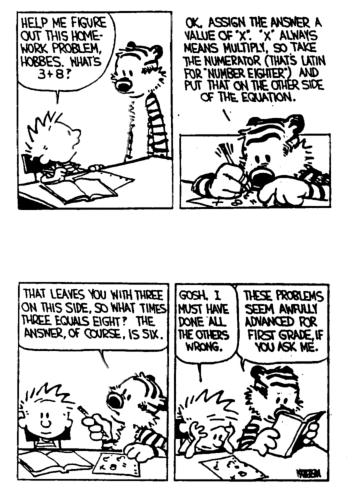
\includegraphics[width=0.7 \linewidth]{3x1-statistiques/sources/cah.jpg}
\end{figure}
\end{multicols}

\end{document}